%\documentclass[fleqn]{book}
\documentclass[11pt]{amsbook}

\usepackage[turkish]{babel}

%\usepackage{../HBSuerDemir}	% ------------------------
\usepackage{../Ceyhun}	% ------------------------
\usepackage{../amsTurkish}


\begin{document}
% ++++++++++++++++++++++++++++++++++++++
\hPage{146}
% ++++++++++++++++++++++++++++++++++++++

değişik ağaç vardır (bu son işlemin 10 tabanına göre yapıldığı gözden kaçmamalıdır).

\begin{multicols}{2}
	
		$R~=Q_{t}~Q_{t}^{'}\\
		\tilde{R}~=Q_{t}^{'}~Q_{t}$\vfill
		\columnbreak$ S~=B_{t}~B_{t}^{'}\\
		\tilde{S}~=B_{t}^{'}~B_{t}$
\end{multicols}

olarak tanımlanan matrislerin taşıdığı anlamın açıklanmasını düşünmek için okuyucuya bırakıyoruz.

\begin{figure}[htb]
	\centering
	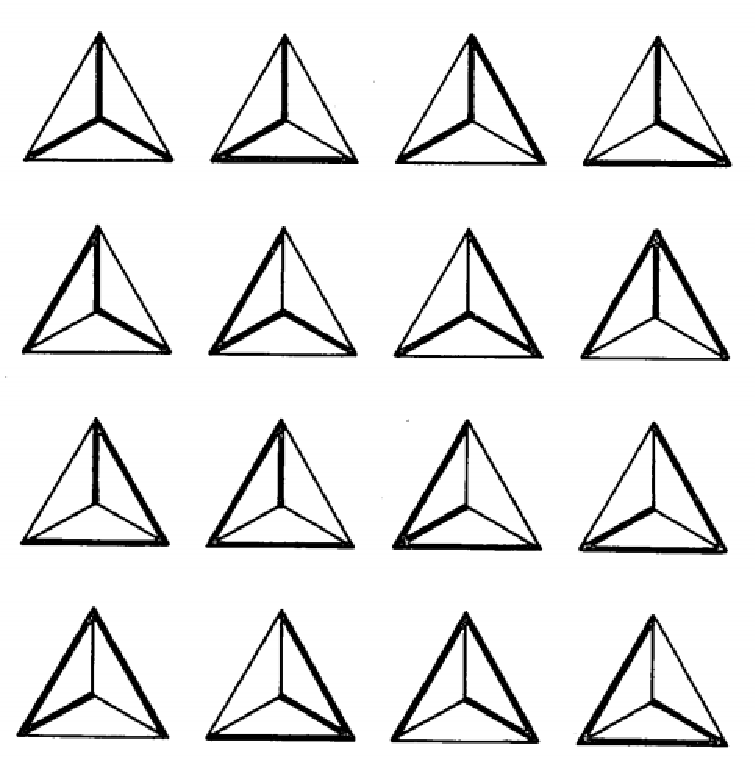
\includegraphics[width=0.45\textwidth]{images/ceyhun-146-fig01}
	\caption{Ç(4,6) daki 16 ağaç.}
	\label{fig:ceyhun-146-fig01}
\end{figure}

\end{document}